
%%%%%%%%%%%%%%%%%%%%%%%%%%%%%%%%%%%%%%%%
\documentclass{paper}
%%%%%%%%%%%%%%%%%%%%%%%%%%%%%%%%%%%%%%%%

% Declare packages in the preamble. 

% Declare some TeX packages needed for graphics. 
\usepackage{graphicx}
\usepackage{epstopdf}
\epstopdfsetup{suffix=}

% Sometimes it helps to use an if statement, 
% if you use the file on multiple platforms. 
% \ifx\pdftexversion\undefined
%     \usepackage[dvips]{graphicx}
% \else
%     \usepackage[pdftex]{graphicx}
%     \usepackage{epstopdf}
%     \epstopdfsetup{suffix=}
% \fi


%%%%%%%%%%%%%%%%%%%%%%%%%%%%%%%%%%%%%%%%
\begin{document}
%%%%%%%%%%%%%%%%%%%%%%%%%%%%%%%%%%%%%%%%

\section{Sample Document}

This is a sample of a document generated automatically from the figures and tables produced by
the script that was used to read in and analyze data.
First, in Section \ref{sec:data}, it describes the data.
Next, in Section \ref{sec:results}, it describes the results of the estimated regression model.
Then, in Section \ref{sec:sensitivity}, it compares the results of several regression models, eliminating one variable at a time.
Finally, Section \ref{sec:conc} concludes. 


\section{Data} \label{sec:data}

Summary statistics for numerical variables are shown in Table \ref{tab:summary} (all figures in millions).

% latex table generated in R 4.0.5 by xtable 1.8-4 package
% Tue Mar 15 12:14:48 2022
\begin{table}[ht]
\centering
\begin{tabular}{rlrr}
  \hline
 & Statistic & house\_price & income \\ 
  \hline
1 & Min. & 0.19 & 0.08 \\ 
  2 & Mean & 0.70 & 0.10 \\ 
  3 & S.D. & 0.18 & 0.01 \\ 
  4 & Max. & 1.09 & 0.13 \\ 
   \hline
\end{tabular}
\caption{Summary of Numeric Variables} 
\label{tab:summary}
\end{table}



Table \ref{tab:earthquakes} shows the frequency of observations in and out of California along with the incidence of earthquakes. Notice that earthquakes have only happened in California.

% latex table generated in R 4.0.5 by xtable 1.8-4 package
% Tue Mar 15 12:14:48 2022
\begin{table}[ht]
\centering
\begin{tabular}{rrr}
  \hline
 & None & Earthquake \\ 
  \hline
Other &  50 &   0 \\ 
  California &  46 &   4 \\ 
   \hline
\end{tabular}
\caption{Earthquake Incidence by State} 
\label{tab:earthquakes}
\end{table}


The correlation matrix of potential variables in the model is shown in Table \ref{tab:corr}.
House prices are positively correlated with income and California but negatively correlated with earthquakes. In the next setion, these variables will be included in a regression model.

              Log. of Price Horsepower         Age Engine Hours
Log. of Price    1.00000000 0.64850242 -0.44054234  -0.04583549
Horsepower       0.64850242 1.00000000  0.03884978   0.37778287
Age             -0.44054234 0.03884978  1.00000000   0.55903832
Engine Hours    -0.04583549 0.37778287  0.55903832   1.00000000




\pagebreak
\section{Empirical Results}  \label{sec:results}


The estimates from the regression model are shown in Table \ref{tab:lm_full_model}.


\begin{table}
\begin{center}
\begin{tabular}{l c}
\hline
 & Model 1 \\
\hline
(Intercept) & $0.173$        \\
            & $(0.096)$      \\
income      & $4.303^{***}$  \\
            & $(0.949)$      \\
in\_cali    & $0.240^{***}$  \\
            & $(0.021)$      \\
earthquake  & $-0.562^{***}$ \\
            & $(0.053)$      \\
\hline
R$^2$       & $0.687$        \\
Adj. R$^2$  & $0.677$        \\
Num. obs.   & $100$          \\
\hline
\multicolumn{2}{l}{\scriptsize{$^{***}p<0.001$; $^{**}p<0.01$; $^{*}p<0.05$}}
\end{tabular}
\caption{Regression Model with All Variables}
\label{tab:lm_full_model}
\end{center}
\end{table}


% Text describing results of regression model. 

%% Regression model description:



The regression model predicts housing prices as follows 
(all figures in millions).
For every one dollar increase in average income, housing prices are expected 
to rise by 4.303. 
If the home is located in California, housing prices are expected 
to be 0.240 higher. 
If there was an earthquake in the zip code, housing prices are expected 
to be -0.562 lower. 
Overall, this model provides a fairly good description with an $R^2$ of 0.677.






\pagebreak
The regression lines are shown in Figure \ref{fig:reg}, with the estimated intercept term for zip codes affected by earthquakes (red), those in the rest of California (green), and the zip codes outside of California.

\begin{figure}
\centering
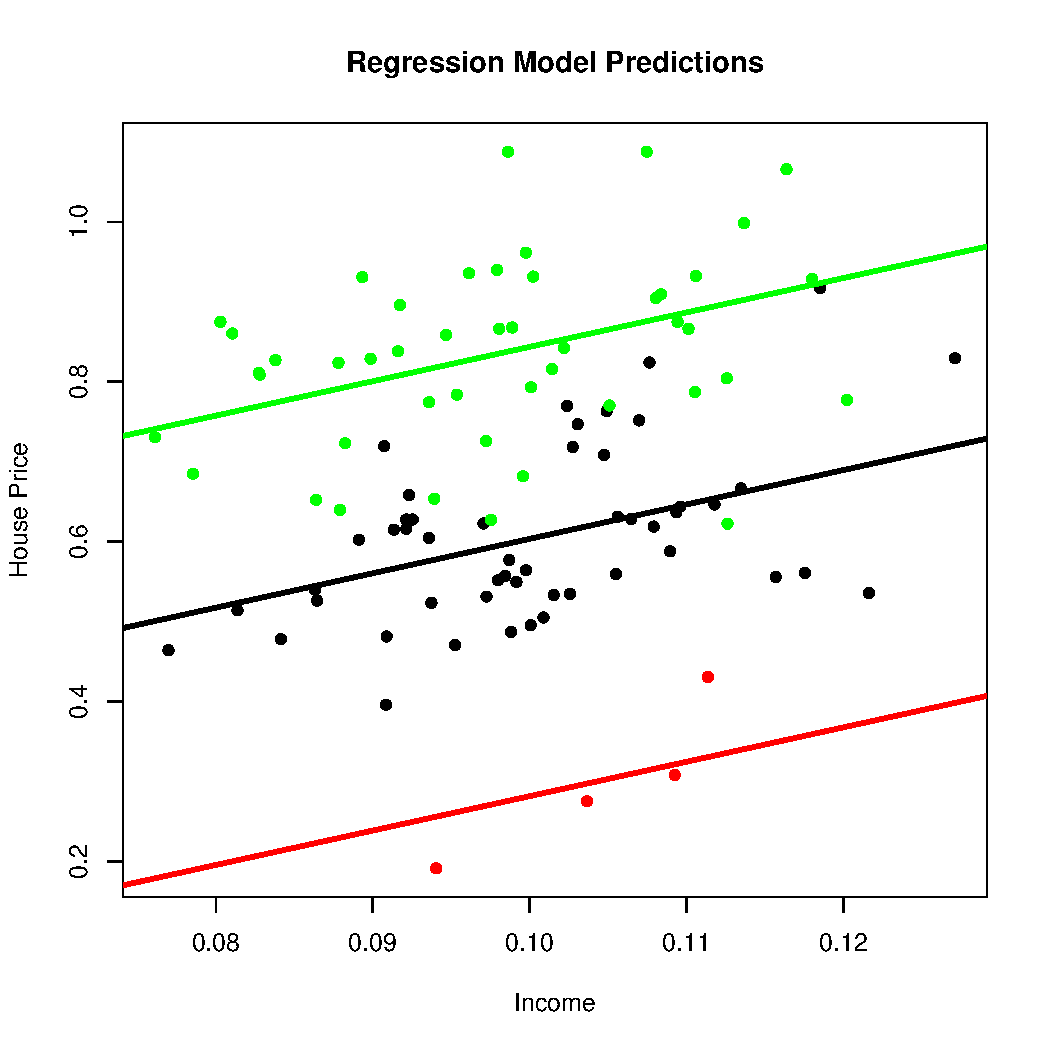
\includegraphics[width=\textwidth]{../Figures/regression.eps}
\caption{Regression Model Predictions}
\label{fig:reg}
\end{figure}


\pagebreak
The predictions are shown in Figure \ref{fig:pred} compared to observed prices.
It is clear that there is a reasonably close relationship between the predictions and the observed prices.

\begin{figure}
\centering
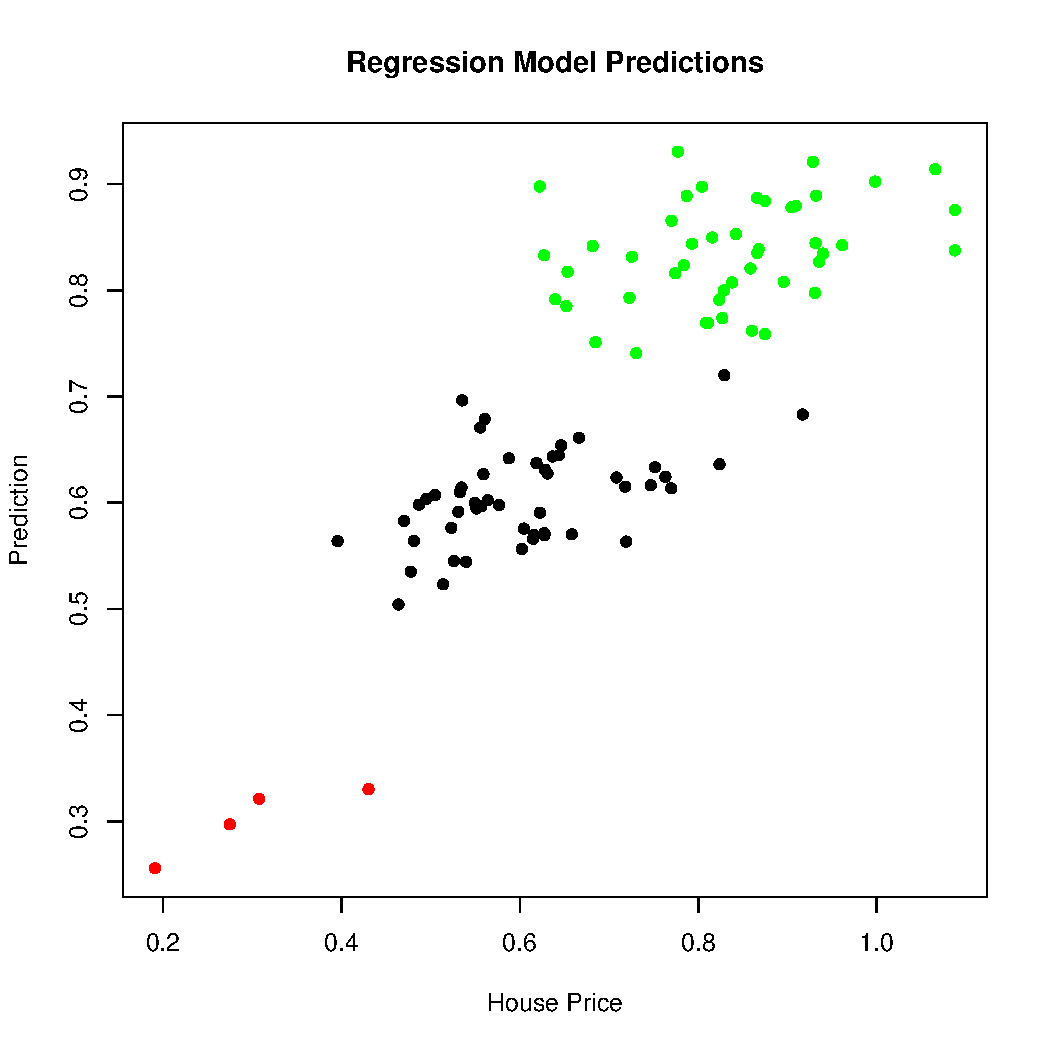
\includegraphics[width=\textwidth]{../Figures/predictions.eps}
\caption{House Prices vs. Predicted Prices}
\label{fig:pred}
\end{figure}



\pagebreak
\section{Sensitivity Analysis}  \label{sec:sensitivity}


The estimates from several regression models are shown in Table \ref{tab:lm_all_models}. 
In each column, one variable was removed at a time
to compare the loss of predictive value.  


\begin{table}
\begin{center}
\begin{tabular}{l c c c}
\hline
 & Model 1 & Model 2 & Model 3 \\
\hline
(Intercept) & $0.173$        & $0.293^{*}$   & $0.472^{**}$ \\
            & $(0.096)$      & $(0.141)$     & $(0.164)$    \\
income      & $4.303^{***}$  & $3.104^{*}$   & $2.275$      \\
            & $(0.949)$      & $(1.384)$     & $(1.642)$    \\
in\_cali    & $0.240^{***}$  & $0.193^{***}$ &              \\
            & $(0.021)$      & $(0.030)$     &              \\
earthquake  & $-0.562^{***}$ &               &              \\
            & $(0.053)$      &               &              \\
\hline
R$^2$       & $0.687$        & $0.317$       & $0.019$      \\
Adj. R$^2$  & $0.677$        & $0.303$       & $0.009$      \\
Num. obs.   & $100$          & $100$         & $100$        \\
\hline
\multicolumn{4}{l}{\scriptsize{$^{***}p<0.001$; $^{**}p<0.01$; $^{*}p<0.05$}}
\end{tabular}
\caption{Several Regression Models}
\label{tab:lm_all_models}
\end{center}
\end{table}


\pagebreak
\section{Conclusion}  \label{sec:conc}

In conclusion, the full model in Table \ref{tab:lm_full_model} is the best.


%%%%%%%%%%%%%%%%%%%%%%%%%%%%%%%%%%%%%%%%
\end{document}
%%%%%%%%%%%%%%%%%%%%%%%%%%%%%%%%%%%%%%%%
